\documentclass[aspectratio=1610]{beamer}
\usetheme{Boadilla}
\usepackage[T1]{fontenc}
\usepackage[utf8]{inputenc}
\usepackage[english]{babel}
\usepackage{graphicx}
\usepackage{hyperref}
\usepackage{url}
\usepackage[T1]{fontenc}
\usepackage{colortbl}
\usepackage{soul,color}
\usepackage{xcolor}
\usepackage{mcode}
\usepackage[utf8]{inputenc}
\usepackage{enumitem}
\usepackage{multicol}
\usepackage{rotating}
\usepackage{framed}
\usepackage{setspace}
\usepackage{geometry}
\usepackage{amsmath}
\usepackage{amsmath}
\usepackage{amssymb}
\usepackage{amsthm}
\usepackage{amsmath,amssymb,lmodern}
\usepackage{tikz}
\usetikzlibrary{
	arrows.meta, % for Straight Barb arrow tip
	fit, % to fit the group box around the central neurons
	positioning, % for relative positioning of the neurons
}

\tikzset{
	neuron/.style={ % style for each neuron
		circle,draw,thick, % drawn as a thick circle
		inner sep=0pt, % no built-in padding between the text and the circle shape
		minimum size=3.5em, % make each neuron the same size regardless of the text inside
		node distance=1ex and 2em, % spacing between neurons (y and x)
	},
	group/.style={ % style for the groups of neurons
		rectangle,draw,thick, % drawn as a thick rectangle
		inner sep=0pt, % no padding between the node contents and the rectangle shape
	},
	io/.style={ % style for the inputs/outputs
		neuron, % inherit the neuron style
		fill=gray!15, % add a fill color
	},
	conn/.style={ % style for the connections
		-{Straight Barb[angle=60:2pt 3]}, % simple barbed arrow tip
		thick, % draw in a thick weight to match other drawing elements
	},
		ncbar angle/.initial=90,
		ncbar/.style={
			to path=(\tikztostart)
			-- ($(\tikztostart)!#1!\pgfkeysvalueof{/tikz/ncbar angle}:(\tikztotarget)$)
			-- ($(\tikztotarget)!($(\tikztostart)!#1!\pgfkeysvalueof{/tikz/ncbar angle}:(\tikztotarget)$)!\pgfkeysvalueof{/tikz/ncbar angle}:(\tikztostart)$)
			-- (\tikztotarget)
		},
		ncbar/.default=0.5cm,
		transition/.style = {rectangle, draw=black!, fill=white, thick, minimum width=1.98cm,
			minimum height = 1.59cm},
		neuron/.style={ % style for each neuron
			circle,draw,thick, % drawn as a thick circle
			inner sep=0pt, % no built-in padding between the text and the circle shape
			minimum size=4.5em, % make each neuron the same size regardless of the text inside
			node distance=1ex and 2em, % spacing between neurons (y and x)
		},
		group/.style={ % style for the groups of neurons
			rectangle,draw,thick, % drawn as a thick rectangle
			inner sep=0pt, % no padding between the node contents and the rectangle shape
		},
		io/.style={ % style for the inputs/outputs
			neuron, % inherit the neuron style
			fill=gray!15, % add a fill color
		},
		conn/.style={ % style for the connections
			-{Straight Barb[angle=60:2pt 3]}, % simple barbed arrow tip
			thick, % draw in a thick weight to match other drawing elements
		},
}
\tikzset{square left brace/.style={ncbar=0.3cm}}
\tikzset{square right brace/.style={ncbar=-0.3cm}}


\title[3rd IMA Conference]{3rd IMA Conference on the Mathematical Challenges \\ of Big Data}
\subtitle {\textcolor{black}{Oral Presentation}}
\author{GABRIELE LA MALFA}
\institute[] % (optional)
{MSc Quantitative Finance\\
	}
\date{11/12/2018}
\begin{document}
{
\begin{frame}
\titlepage 
\end{frame}
}
{
\begin{frame}
\frametitle{Abstract}
	\begin{itemize}
		\item \textcolor{red}{Title:}\\ Time Series Forecasting and Anomaly Detection using Machine
		Learning Algorithms: a Comparison of Performances
		\item \textcolor{red}{Topic:}\\Time Series Forecasting and Anomaly Detection using Sequentially Discounting Autoregressive algorithm (SDAR) and Long Short-Term memory Recurrent Neural Network (LSTM RNN algorithm)
		\item \textcolor{red}{Keywords:}\\ Time Series Analysis, Machine Learning, Outliers Detection, Forecasting, Simulation
	\end{itemize}
\end{frame}
}

\begin{frame}
\frametitle{SDAR Algorithm: Sequentially Discounting AR Model}
SDAR algorithm is a statistical based algorithm, which permits to learn a statistical behaviour of data provided. \\
Data behaviour is called "statistical regularity". Once the statistical behaviour has been learnt, data can be compared to it and therefore identified through different criteria such as outliers or not.
\end{frame}
\begin{frame}
\frametitle{SDAR Algorithm: Characteristics}
\begin{itemize}
\item The process implemented is an online algorithm. This allows to immediately determine whether or not a given subset of points represents outliers.\\
\item Another feature of the model is the ability to detect anomalies even in the presence of a non-stationary process (stationarity is often considered optimal for working with other models)\\
\item SDAR model as presented in [1], assumes a Gaussian Mixture as a statistical model for continuous variables.\\
The AR algorithm permits to update the parameters of the Gaussian distribution, applying a discounting effect on past data.
\end{itemize}
\end{frame}
\begin{frame}
	\frametitle{SDAR Algorithm: Characteristics}
Given that the Probability Density Function is a Multivariate Gaussian function as follows:
\begin{eqnarray}
p(x_t|x^{t-1}_{t-k}:\theta)=\frac{1}{\sqrt{(2\pi)^{k/2}|\Sigma|}}exp(-\frac{1}{2}(x_{t}-\omega)^T\Sigma^{-1}(x_{t}-\omega)
\end{eqnarray}
$\hat{x_t}$ and $\hat{\Sigma}$ are the parameters of the Multivariate Gaussian.
\begin{eqnarray}
\hat{x_t}=\hat{\omega}(x^{t-1}_{t-k}-\hat{\mu})+\hat{\mu}
\end{eqnarray}
\begin{eqnarray}
\hat{\Sigma}=(1-r)\hat{\Sigma}+r(x_t-\hat{x_t})(x_t-\hat{x_t})^T
\end{eqnarray}
$\hat{x_t}$ is the weighted distance of each $x_t$ $\in{k}$ from the updated mean $\hat{\mu}$, plus the updated mean $\hat{\mu}$.
\\$\hat{\mu}$ is updated as follows:
\begin{eqnarray}
\hat{\mu}=(1-r)\hat{\mu}+rx_t
\end{eqnarray}
\end{frame}

\begin{frame}
	\frametitle{SDAR Algorithm: Characteristics}
	Covariance function ($C$) is a weighted sum of the previous covariances between steps belonging to $k$ and $\omega_i$ (\textit{weights} variable in the implementation) are the solutions to equation (5) and they are used to compute $\hat{x_t}$ in equation (2).
\begin{eqnarray}
C_J=\sum_{i=1}^k\omega_iC_{j-i}\hspace{0.35cm}(j=1,...,k)
\end{eqnarray}
Using a loop \textit{for j in range (k)}, $C_j$ is computed as follows:
\begin{eqnarray}
C_J = (1-r)C_j+r(x_t-\hat{\mu})(x_{t-j}-\hat{\mu})^T
\end{eqnarray}
\end{frame}
\begin{frame}
	\frametitle{Scoring: Outliers and Change Points Detection}
	For outliers detection, the following algorithm is proposed:
	\begin{eqnarray}
	Score(x_t)= -logp_{t-1}(x_t),
	\end{eqnarray} 
	which is the loss (logarithmic loss) performed regarding the point $x_t$, using a prediction based on the probability density at time $t-1$.
	\\The following formula computes the change point scoring: 
	\begin{eqnarray}
	Scoring(T)= 1/T\sum_{i=t-T+1}^t score(x_i)
	\end{eqnarray}
	Through algorithm (8), a time series of averaged scores is obtained. This time series is used in SDAR to calculate new distribution parameters ($x_{hat}$ and $sigma_{hat}$) and a sequence of pdf denoted as $q_t$ with $t=1,2...t$.\\
	When $T_1$ is set as the new window constant, the new score is calculated as follows:
	\begin{eqnarray}
	Score(t)= 1/T'\sum_{i=t-T'+1}^t (-lnq_{i-1}(y_i))
	\end{eqnarray}
\end{frame}
\begin{frame}
	\frametitle{Test: Data}
	To perform test section, two dataset of the same index are used:
	\begin{itemize}
		\item TOPIX year: 1985-1995
		\item FTSEeurofirst 300 year: 2007-2018
	\end{itemize}
TOPIX and FTSEEurofirst 300 data are taken from S\&P Capital IQ  and they are normalized according to min-max normalization.
\\Change point detection is performed using formulae (8) and (9).\\
SDAR parameters are: $r=0.005$ and $k=15$. 
\\For change point detection, $T=5$ and $T_1 = 5$.
	
\end{frame}
\begin{frame}
	\frametitle{Figure 1: TOPIX}
	\begin{figure}[!h]
		\centering
		{\includegraphics[scale=0.55]{TOPIX_Index}}
		\caption{Change Point Detection TOPIX 1985-1995 \label{t1v2}}
	\end{figure}
\end{frame}
\begin{frame}
	\frametitle{Figure 2: FTSEEurofirst 300}
	\begin{figure}[!h]
		\centering
		{\includegraphics[scale=0.55]{FTSE_EUROFIRTS_300}}
		\caption{Change Point Detection FTSEeurofirst 300 2007-2018 \label{t1v2}}
	\end{figure}
 	\end{frame}
 	\begin{frame}
 		\frametitle{LSTM RNN: Characteristics}
 		Recurrent Neural Networks (RNNs) are a sequence of Neural Networks (NNs) $N_1,N_2, ..., N_n$ arranged each at every single step of a discrete process.\\
 		Recurrent Neural Networks are able to take a sequence of input-values $x_1, ..., x_n$ one at a time leading the information along the process.\\ 
 		Inputs are processed by the neural networks and a vector of parameters (weights) is updated. These parameters contain the information coming from the past Neural Networks: in this way the information flows through the Neural Networks.
 	\end{frame}
\begin{frame}
\frametitle{LSTM RNN: Forward Propagation}
RNNs forward propagation process is formalized as follows:
\begin{eqnarray}
a_{t} = f(W_{aa} a_{t-1}+W_{ax}x_{t}+b_a)
\end{eqnarray}
\begin{eqnarray}
\hat{y}_{t} = g(W_{ya}a_{t}+b_y)
\end{eqnarray}
\begin{itemize}
\item Where: $a$ is the activation function of the next NN; 
\item $W_{aa}$, $W_{ax}$, $W_{ya}$ are respectively the weights related to the next activation function, the NN inputs and the NN output;
\item $x_{t}$ is the input of the NN at step $t$;
\item $f(),g()$ are a non-linear function (in literature hyperbolic tangent and softmax are respectively used as $f$ and $g$ function);
\item $\hat{y}_{t}$ is the output of the NN at step $t$;
\item $b_a$ and $b_y$ are the biases of activation functions and outputs 
\end{itemize}	
\end{frame}
\begin{frame}
\frametitle{LSTM RNN: Loss}
After the computations of the forward propagation, it is necessary to calculate the Loss of the model which is translated in the summation of the losses of the model for each training step and each pair of values of the sequence $(x_1, y_1), (x_2, y_2), (...), (x_n, y_n)$.\\
The single-step loss is: $L_t(\hat{y_t}, y_t)$.\\
The overall loss is: $L(\hat{y},y) = \sum_{t=1}^t L_t$.
\\The loss of the model is calculated in accordance with the intended purpose. Generally, the loss is calculated as the "distance" between the prediction $\hat{y}$ coming from the networks' computations and the label of the supervised model $y$.
\end{frame}
\begin{frame}
\frametitle{LSTM RNN: Information and Backpropagation}	
There may be different architectures for the RNNs: for example the hidden layer $h_t$ could depend on the hidden layer $h_{t-1}$ at the previous step or imply in the calculation also the output $y_{t-1}$ of the previous step. The different architecture defines the passage of information between one RNN cell and another.\\
In the deep neural networks, even if the weights are shared, the way in which the passage of the information happens turns out to be very difficult to be interpreted: the parameters to be updated are many and their change often makes lose of interpretability so much that often the neural networks are used as black boxes.\\
Backpropagation is used to update the parameters of the RNN. It is often based on an optimization process, calculating the partial derivatives of the Loss with respect to the weights ($W_{aa}$, $W_{ax}$, $W_{ya}$), calculating the gradient of the loss function and finally using an optimization method to minimize the loss function. 
\end{frame}
\begin{frame}
\frametitle{LSTM RNN: Different RNN Architectures}	
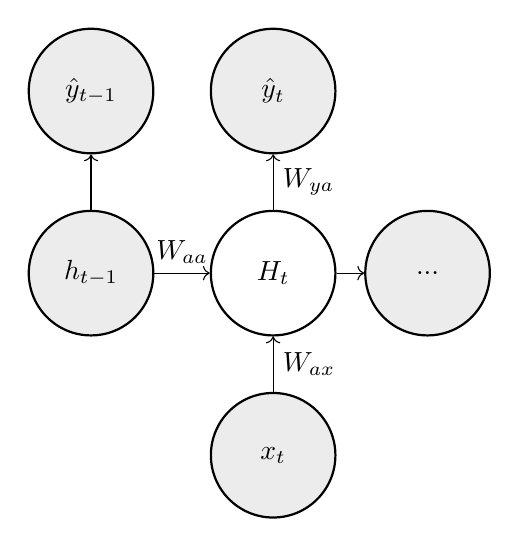
\begin{tikzpicture}
\node[neuron] (htn) {$H_t$};
\node[io,left=2em of htn] (ht-1) {${h}_{t-1}$};
\node[io,above=2em of ht-1] (yt-1) {$\hat{y}_{t-1}$};
\node[io,above=2em of htn] (yt) {$\hat{y}_t$};
\node[io,below=2em of htn] (vt) {${x}_t$};
\node[io,right=1em of htn] (ht+1) {$...$};
\draw[->] (ht-1) -- node[align=center,above] {$W_{aa}$} (htn);
\draw[->] (ht-1) -- node[align=center,above] {$$} (yt-1);
\draw[->] (htn) -- node[align=center,right] {$W_{ya}$} (yt) ;
\draw[->] (vt) -- node[align=center,right] {$W_{ax}$} (htn);
\draw[->] (htn) -- node[align=center,above] {$$} (ht+1);
\end{tikzpicture}
\hspace{2cm}
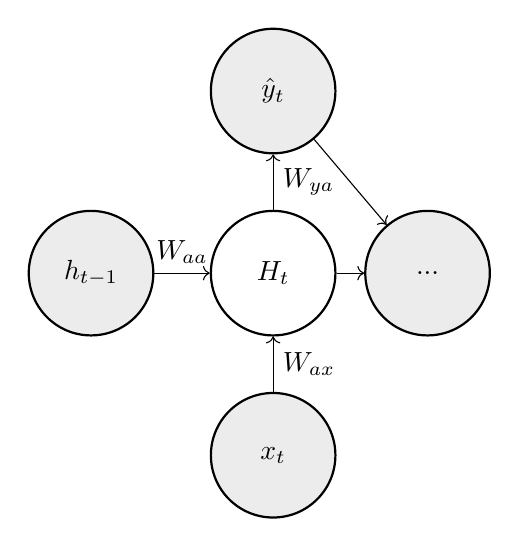
\begin{tikzpicture}
\node[neuron] (htn) {$H_t$};
\node[io,left=2em of htn] (ht-1) {${h}_{t-1}$};
\node[io,above=2em of htn] (yt) {$\hat{y}_t$};
\node[io,below=2em of htn] (vt) {${x}_t$};
\node[io,right=1em of htn] (ht+1) {$...$};
\draw[->] (ht-1) -- node[align=center,above] {$W_{aa}$} (htn) ;
\draw[->] (htn) -- node[align=center,right] {$W_{ya}$} (yt) ;
\draw[->] (vt) -- node[align=center,right] {$W_{ax}$} (htn);
\draw[->] (htn) -- node[align=center,above] {$$} (ht+1);
\draw[->] (yt) -- node[align=center,above] {$$} (ht+1);
\end{tikzpicture}
\end{frame}
\begin{frame}
\frametitle{LSTM RNN: High Temporal Distance Relationship Learning}
Parameter updatings depend on how the loss is optimized and how the gradient converges to the minimum in backpropagation: weights update is proportional to the partial derivatives of the loss function.\\
There may be two pathological situations:
\begin{itemize}
	\item Vanishing gradients: if the weights are small, the gradient convergence to the minimum may be very small or stop.
	\item Exploding gradients: if the weights are large, the learning mechanism may diverge.
\end{itemize}
LSTM networks implement a system of gates (Input Gate, Output Gate and Forget Gate) leading the activation or the inhibition of the information in the cell memory:
\begin{itemize}
	\item Input Gate: the memory cell retains the previous state.
	\item Forget Gate: resets the state of the cell.
	\item Output Gate: it enables the information to be carried on or not.
\end{itemize}
LSTM model permits to manage the information and the overall recurrent process for a long time series.
\end{frame}
\begin{frame}
	\frametitle{LSTM: Architecture}
	\centering
	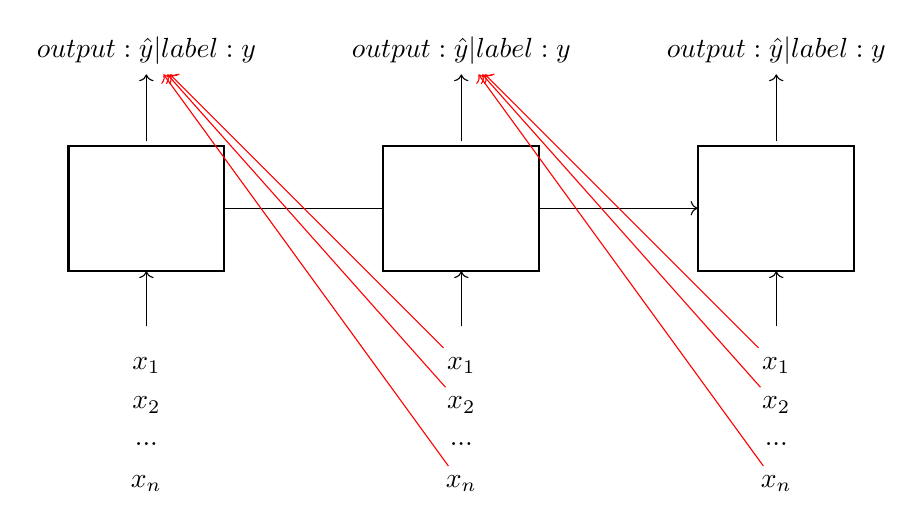
\begin{tikzpicture}
	\node at (1.15, -2.5) (O) {$output: \hat{y}|label: y$};
	\node at (5.15, -2.5) (P) {$output: \hat{y}|label: y$};
	\node at (9.15, -2.5) (Q) {$output: \hat{y}|label: y$};
	
	\node at (1.15, -6.5) () {$x_1$};
	\node at (1.15, -7) () {$x_2$};
	\node at (1.15, -7.5) () {...};
	\node at (1.15, -8) () {$x_n$};
	\node at (5.15, -6.5) (T) {$x_1$};
	\node at (5.15, -7) (U) {$x_2$};
	\node at (5.15, -7.5) () {...};
	\node at (5.15, -8) (V) {$x_n$};
	\node at (9.15, -6.5) (X) {$x_1$};
	\node at (9.15, -7) (Y) {$x_2$};
	\node at (9.15, -7.5) () {...};
	\node at (9.15, -8) (W) {$x_n$};
	\node[transition] (n1) at (1.15, -4.5) {};
	\node[transition] (n2) at (5.15, -4.5) {};
	\node[transition] (n3) at (9.15, -4.5) {};
	
	\coordinate (G) at (2.15, -4.5);
	\coordinate (R) at (4.15, -4.5);
	\draw [black, -] (G) -- (R);
	
	\coordinate (G) at (6.15, -4.5);
	\coordinate (R) at (6.65, -4.5);
	\draw [black, -] (G) -- (R);
	
	\coordinate (G) at (7.65, -4.5);
	\coordinate (R) at (8.15, -4.5);
	\draw [black, ->] (G) -- (R);
	
	\coordinate (G) at (6.65, -4.5);
	\coordinate (R) at (7.65, -4.5);
	\draw[black, -] (G) -- (R);
	
	\coordinate (A) at (1.15, -3.65);
	\coordinate (B) at (1.15, -2.8);
	\draw [black, ->] (A) -- (B);
	\coordinate (C) at (5.15, -3.65);
	\coordinate (D) at (5.15, -2.8);
	\draw [black, ->] (C) -- (D);
	\coordinate (E) at (9.15, -3.65);
	\coordinate (F) at (9.15, -2.8);
	\draw [black, ->] (E) -- (F);
	
	\coordinate (G) at (1.15, -6);
	\coordinate (H) at (1.15, -5.3);
	\draw [black, ->] (G) -- (H);
	\coordinate (I) at (5.15, -6);
	\coordinate (L) at (5.15, -5.3);
	\draw [black, ->] (I) -- (L);
	\coordinate (M) at (9.15, -6);
	\coordinate (N) at (9.15, -5.3);
	\draw [black, ->] (M) -- (N);
	
	\draw [red, ->] (T) -- (O);
	\draw [red, ->] (U) -- (O);
	\draw [red, ->] (V) -- (O);
	
	\draw [red, ->] (X) -- (P);
	\draw [red, ->] (Y) -- (P);
	\draw [red, ->] (W) -- (P);
	
	
	\end{tikzpicture}
	
	The basic idea is that the RNN (LSTM) learns the weights using the next step input $x_{t+1}$ as the label of the previous step $t$. The error is the difference between the prediction $\hat{y_t}$ and the label $y$ (next step input $x_{t+1}$). 
\end{frame}
\begin{frame}
\frametitle{Test: Data}
To perform test section, three datasets are used:
\begin{itemize}
	\item TOPIX year: 1985-1995
	\item FTSEeurofirst 300 year: 2007-2018
	\item ABSKF (FTSEeurofirst 300) year: 2007-2018
\end{itemize}
The whole historical series relative to the three datasets, is subdivided in train, validation and test according to different percentages established by the experiments.
\end{frame}
\begin{frame}
\frametitle{Anomaly Detection with LSTM}	
The following procedure is used to do anomaly detection with the LSTM model:
\begin{itemize}
	\item 1.Training of the model on  train part of the dataset;
	\item 2.Error computation on validation part as the difference between the label and the prediction;
	\item 3.Assuming that the errors are distributed according to a Gaussian distribution, the parameters $\mu$ and $\theta$ are fitted on validation part with MLE;
	\item 4.With new data coming from the test part, once the test errors are estimated, we calculate the probability $p(t)$ of observing each error according to the previous Gaussian;
	\item 5.If $p(t)$ is lower than a fixed threshold $\tau$, then we are in presence of an anomaly.
	 
\end{itemize}
\end{frame}
\begin{frame}
	\frametitle{Figure 3: TOPIX}
	\begin{figure}[!h]
		\centering
		{\includegraphics[scale=0.45]{LSTM_TEST_TOPIX}}
		\caption{Change Point Detection \label{t1v2}}
	\end{figure}	
\end{frame}
\begin{frame}
	\frametitle{Figure 4: FTSEeurofirst 300}
	\begin{figure}[!h]
		\centering
		{\includegraphics[scale=0.45]{LSTM_TEST_FTSE_EUROFIRST_300}}
		\caption{Change Point Detection \label{t1v2}}
	\end{figure}	
\end{frame}
\begin{frame}
	\frametitle{Figure 5: ABSKF}
	\begin{figure}[!h]
		\centering
		{\includegraphics[scale=0.6]{LSTM_TEST_ABSKF}}
		\caption{Change Point Detection \label{t1v2}}
	\end{figure}	
\end{frame}
\begin{frame}
	\centering
	\begin{LARGE}
	A special thanks to my brother Emanuele for his contributions and his support so that this first presentation of mine can be presented here
	\end{LARGE}
\end{frame}
\begin{frame}
	\centering
	\begin{Huge}
		Thank you for your attention
	\end{Huge}
\end{frame}
\begin{frame}
	\frametitle{Bibliography}
	\begin{thebibliography}{References}
		\bibitem-Takeuchi, J, Yamanishi, K, A unifying framework for detecting outliers and change points from time series, \textit{IEEE Transactions on Knowledge and Data Engineering}, Volume 18, Issue 4, April 2006.
		\bibitem-Malhotra,P, Vig, L, Shroff, G, Agarwal, P, Long Short Term Memory Networks for Anomaly Detection in Time Series, \textit{European Symposium on Artificial Neural Networks, Computational Intelligence
			and Machine Learning}, Bruges (Belgium) 22-24 April 2015.
		
	\end{thebibliography}
\end{frame}
\end{document}